\section{Naive Example}
Looking back at \cref{fig:running-example}, this example was created by human hands. In its design there is an attempt to maximize throughput by creating seperate lines for different types of items and to increase throughput by using additional modules. Now, how would a computer given a set of modules and an same order arrive at the same configuration?

To start off, we need some initial configuration, from which we can start the search towards the optima. We choose this configuration to be naively constructed, as it will be easy to generate. Let us say that we are given the same modules as in \cref{fig:running-example}. In addition, we are supposed to produce three types of items, a doll, a rocking horse and a wooden sword as described in \cref{fig:toy-recipes}. Obviously, these items can be produced by the running example. The same is true for the naivley constructed configuration shown in \cref{fig:trivial-example}.  

\begin{figure}[H]
\centering
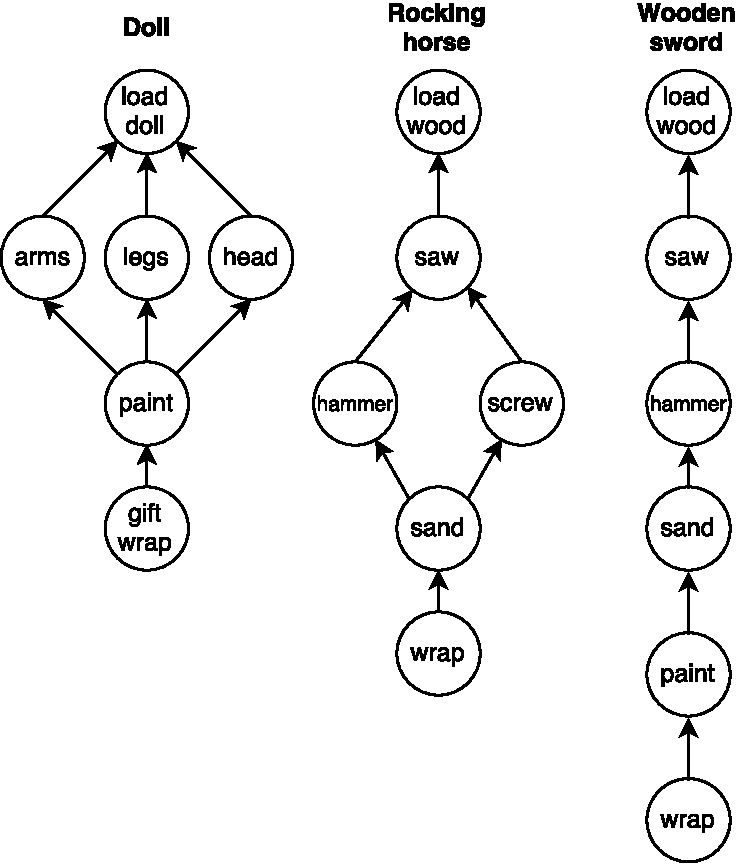
\includegraphics[width=\textwidth]{toyrecipes.pdf}
\caption{Acyclic dependency graphs describing three item types.}
\label{fig:toy-recipes}
\end{figure}

\begin{figure}[H]
\centering
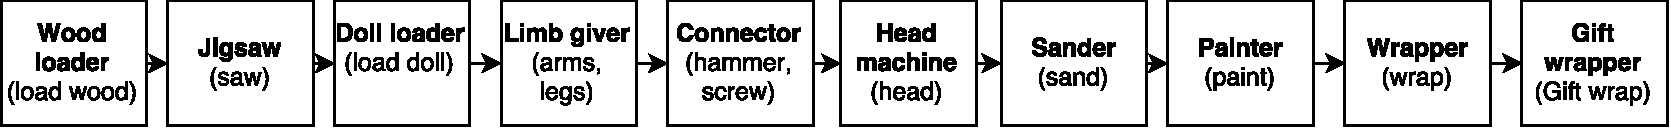
\includegraphics[width=\textwidth]{trivialexample.pdf}
\caption{A trivial configuration of a toy factory layout}
\label{fig:trivial-example}
\end{figure}


This naive configuration is obviously a poorer choice. In the man-made configuration no item has to pass through a module, where it is not worked upon. At least, when excluding the transport module. We originally got around this issue by producing items on separate lines. In comparison, the trivial configuration is made of a single line.

In addition the trivial example uses the minimal amount of modules needed to process our orders. This means that it does not try to increase throughput by adding additional modules to the configuration. 

Yet, the advantage of the trivial example is that it is very simple to generate using a computer. This can not be said for the man-made configuration. To produce the naive example, we have to compose the three graphs in \cref{fig:toy-recipes}. On the resulting dependency graph, we then perform a topological sort. This gives us an ordered list of works, which we can then use as a blueprint to place down modules in a line, connecting them from left to right.

A dependency graph may of course have several topological sorts. Because of this we could just generate a configuration for each of these sorts. Each of these candidate solutions can then be set up in our UPPAAL model, and we can find the execution time of their fastest trace. The configuration with the fastest trace is then deemed the best fitting candidate.  Yet, again this configuration would most likely still be poor compared to the one we created ourselves.

Because of this, we want to define ways in which we from a naive single line configuration are able to transform into more complex configurations, which may be better at producing the given order. In the rest of this chapter we will formally define tranformation rules, which allow us to do this. 







